\chapter{Stakeholder analysis}
\label{chapter:stakeholders}

This chapter explains the stakeholders related to Rio Paraná Guazú, focusing on their interests in sand dredging activities. The interests and goals of the stakeholders are explained, and a power versus interest matrix evaluates their relevance to the project.

\section{Stakeholders interest and power}

All relevant stakeholders were identified for this project, some suggested by INA staff and others through further investigation. The complete list is in Table \ref{tab:stakeholders} and will be discussed in the following sections. The stakeholder descriptions are in Table \ref{tab:stakeholders-description}, and their interests and goals in Table \ref{tab:stakeholders-interests-goals}.

\subsubsection{Stakeholders}

\begin{table}[H]
\centering
\begin{tabularx}{\linewidth}{p{3.5cm}X} % narrower first column
\toprule
\textbf{Stakeholders} & \textbf{Role} \\
\midrule
Dredgers & Extraction of sand and gravel from shallow river areas. \\
\midrule
Dredging companies & Large-scale extraction and commercial sale of sand. \\
\midrule
Prefectura Naval Argentina (PNA) & Protection of rivers and maritime territory, and functions as coast guard and river police. \\
\midrule
Agencia Nacional de Puertos y Navegación (ANdPyN) & Oversight of signalling systems, dredging operations, and maintenance of the Main Waterway. \\
\midrule
Ports & Handling, storing, and trading of goods and dredged material. \\
\midrule
Fishermen & Artisanal and independent fishing activities for local and regional markets. \\
\midrule
NGOs & Non-profit organizations advocating for environmental protection and community interests. \\
\midrule
Landowners & - \\
\midrule
Filmmakers & Filmmakers documenting trade and social impacts of the Paraná–Paraguay waterway. \\
\bottomrule
\end{tabularx}
\caption{Potential stakeholders and their roles}
\label{tab:stakeholders}
\end{table}

\subsubsection{Stakeholders description}

\begin{table}[H]
\centering
\begin{tabularx}{\linewidth}{p{3.5cm}X} % fixed width first column
\toprule
\textbf{Stakeholders} & \textbf{Description} \\
\midrule
Dredgers & Dredgers are local boats that extract sand and gravel from the Paraná Guazú, ranging from small independent vessels to organized groups of boats (areneros) and larger hopper ships. They operate mainly in shallow areas where simple extraction methods are possible, transporting the material to nearby ports such as Ibicuy or Brazo Largo. \\
\midrule
Dredging companies & Dredging companies operate larger vessels and equipment to extract and sell sand from the Paraná Guazú. Unlike small-scale dredgers, these companies are commercially organized and supply sand to construction, industrial, and infrastructure markets. \\
\midrule
Prefectura Naval Argentina (PNA) & Prefectura Naval Argentina (PNA) serves as Argentina’s coast guard and river police, operating under the Ministry of National Security. It is responsible for protecting rivers and maritime territory, ensuring safety, security, and regulatory compliance. In the Paraná Guazú, PNA plays a key role in monitoring dredging activity and maintaining lawful use of waterways. \\
\midrule
Agencia Nacional de Puertos y Navegación (ANdPyN) & Agencia Nacional de Puertos y Navegación is the authority in charge of implementing and controlling the signalling system, as well as overseeing dredging and maintenance along the Main Waterway, which includes the Paraná Guazú. As an independent agency within the Ministry of Economics, it ensures navigational safety and operational continuity of ports and waterways. \\
\midrule
Ports & Ports serve as key logistical hubs for handling and storing goods extracted or transported along the Paraná Guazú. They provide the facilities where dredged sand is unloaded and traded, connecting local extraction activities with broader commercial markets. Their role is essential in enabling the flow of materials and supporting both regional trade and industrial supply chains. \\
\midrule
Fishermen & Fishermen on the Paraná Guazú depend on the river’s abundant fish resources, particularly migratory species such as sábalo, surubí, boga, pacú, and dorado. Most are independent artisanal fishers, selling their catch through middlemen, freezing plants, or informal markets. Although associations exist in the region, they hold little influence in decision-making over river use and management. \\
\midrule
NGOs & Non-governmental organizations play a role in monitoring the social and environmental impacts of activities along the Paraná Guazú. They advocate for sustainable river management, community interests, and the protection of ecosystems affected by dredging and trade. Their involvement adds external oversight and pressure on both companies and authorities to adopt responsible practices. \\
\midrule
Landowners & - \\
\midrule
Filmmakers & Alejo Di Risio is a filmmaker who directed a documentary on the Paraná–Paraguay waterway, focusing on the impacts of trade along the river system. His work highlights the economic and social dimensions of waterway use, bringing public attention to stakeholders and their activities. He was also contacted during this study to provide additional insights into stakeholders and businesses connected to the waterway. \\
\bottomrule
\end{tabularx}
\caption{Stakeholder descriptions}
\label{tab:stakeholders-description}
\end{table}

\subsubsection{Stakeholders interest and goal}

\begin{table}[H]
\centering
\begin{tabularx}{\linewidth}{p{3.5cm}XX}
\toprule
\textbf{Stakeholders} & \textbf{Interest} & \textbf{Goal} \\
\midrule
Dredgers & Access to shallow river areas for sand extraction. & Sell extracted sand to nearby ports and local markets for income. \\
\midrule
Dredging companies & Large-scale extraction and commercialization of sand. & Maintain profitable operations by supplying construction and industrial demand. \\
\midrule
Prefectura Naval Argentina (PNA) & Safety and security of rivers and maritime territory. & Enforce regulations, monitor dredging, and ensure lawful use of waterways. \\
\midrule
Agencia Nacional de Puertos y Navegación (ANdPyN) & Oversight of navigation safety and waterway infrastructure. & Implement signalling systems, maintain dredging operations, and secure efficient transport. \\
\midrule
Ports & Handling and trading of goods and dredged material. & Strengthen logistical capacity and support regional trade flows. \\
\midrule
Fishermen & Access to fish resources in the Paraná Guazú. & Sustain livelihoods through artisanal fishing and market sales. \\
\midrule
NGOs & Environmental protection and community rights. & Promote sustainable river management and hold stakeholders accountable. \\
\midrule
Landowners & - & -\\
\midrule
Filmmakers & Research and documentation of waterway dynamics. & Raise awareness through film on trade, impacts, and stakeholder activities. \\
\bottomrule
\end{tabularx}
\caption{Stakeholders interest and goal}
\label{tab:stakeholders-interests-goals}
\end{table}

\section{Stakeholders management}

After identifying stakeholders, it is important to evaluate their power and interest in the project. This is visualized using a power versus interest matrix, with power on the vertical axis and interest on the horizontal axis. Analyzing this matrix informs strategies to approach specific stakeholders.

\subsubsection{Power vs. Interest}

The power vs. interest matrix is divided into four parts. These parts can be seen in Figure \ref{fig:power-interest} and represent the amount of power and interest with low and high. High power and high interest are stated as the key player, and these will be of most importance to the project. Next, the quadrant with low power and high interest is stated as subjects, and the ones with high power but low interest are seen as the context setters. The context setters are not close to the project; however, when they want, they can be of high importance. The quadrant of low power and low interest is seen as the crowd, and they are not interested in the project.



\begin{figure}[H]
    \centering
    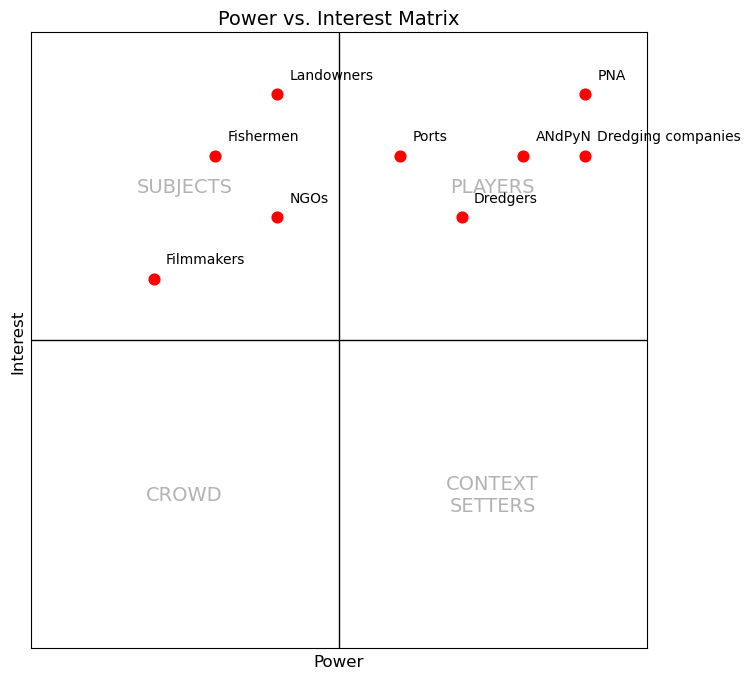
\includegraphics[width=0.70\linewidth]{figures/PowerVSInterest.png}
    \caption{Power versus Interest matrix}
    \label{fig:power-interest}
\end{figure}

\section{Conclusion}

% \section{Dredgers (LOCAL??)}
% The first dominant group of stakeholders are the dredgers.These include the local boats used in the area to extract sand and gravel from the river. There are several different types of dredgers ranging from small independent boats, to groups of small boats that work for the same employer (ARENEROS??), or big extracting ships commonly referred to as 'hoppers'. In the area of interest, the Paraná Guazú from Ibicuy to Brazo Largo, the most common dredgers are: (ARENEROS, INDEPENDENT BOATS). 

% Currently there are 2 active boats in the zone of the Rio Paraná Guazú of interest, and (QUITE A LOT MORE IN IBICUY?? FROM INTERVIEW), as mentioned in the previous Chapter. (DREDGING ACTIVITY AANGEVEN WELKE BOTEN, MAPS MET HEEN EN TERUG REIS, DATA , ETC)

% Their interest in the Rio Paraná Guazú is to extract the sand in locations of the river that are shallow since they do not possess any technology to mine the sand from deep. Once this water mixed sand is lifted onto the boat, they transport it to the nearest ports, Ibicuy or Brazo Largo. They sell their sand to the highest bidder which can be for (PURPOSES FROM INTERVIEW).


% \section{BIG Dredging Companies?}
% because they buy the sand and employ the areneros?
% The Dredging companies active in the Rio Paraná Guazú are :
% (EERST KIJKEN OF YPF, JAn de NUl, etc hierbij kan worden betrokken of niet)


% \section{Prefectura Naval Argentina}
% The Prefectura Naval Argentina (PNA), is the National Naval Prefecture of the Rio Paraná. Therefore, they are also active in the Paraná Guazú and our area of surveillance. 
% It is in their interest to protect the Rio Paraná Guazú from criminal activities. These can 

% \section{Agencia Nacional de Puertos y Navegación}
% The Agencia Nacional de Puertos y Navegación (ANPYN), or the National Agency of Ports and Navigation, was created on January 6, 2025 by a merger of the Undersecretariat of Ports, Waterways and Merchant Marine and the General Port Administration. Since then, the agency has taken over the tasks of the two former entities and is now responsible for policies concerning ports, waterways and river and maritime transport. As such, keeping the Vía Navegable Troncal (VNT), Argentina's main waterway, navigable for ships is an important task for the agency. To achieve this, they regulate dredging and sand mining contracts and oversee compliance with the relevant regulations \autocite{boletinoficialdelarepublicaargentinaAgenciaNacionalPuertos2025}.

% \section{Ports}
% In the researched area there are two strategic port locations that play a key role in the sand extraction.

% \subsection{Guazú}
% ?
% \subsection{Ibicuy}
% ?

% \section{Fishermen}
% Fischermen is another stakeholder group relevant for this study. The Rio Paraná Guazu is used by a lot of people for its high concentration of fish. 

% The artisanal fisheries play an economic role as most of the harvest is sold to middlemen, freezing plants, or in informal markets. Of particular interest are long-range migratory species such as sábalo (Prochilodus lineatus), surubí (Pseudoplatystom corruscans, P. reticulatus), boga (Megaleporinus obtusidens), pacú (Piaractus mesopotamicus), and dorado (Salminus brasiliensis), that support artisanal, recreational, and subsistence fisheries, as observed in other large neotropical rivers, \autocite{assessment of sabalo}, \autocite{fishers' knowledge}

% the fischermen in the region of interest are mostly independent. Even though there exists such thing as fischermen associations in the Rio Paraná Guazú, they are not influencial 



% \section{NGO's}
% even wachten tot ik een nice milieu organisatie vind.

% \section{Agua y Saneamientos Argentinos}
% Even wachten tot interview met hun, kijken of ze wel relevant zijn


% \section{Filmmaker}

% When researching for the stakeholders which were relevant for the analysis. We stumble upon an article on a film that was made on the Parana-Paraguay waterway. In this documentary, the focus is on the impact of the trade happening on the Parana-Paraguay waterway. The documentary is made by filmmaker Alejo Di Risio, who was contacted through journalist Matias Avramow for any additional information about stakeholders and business related to the waterway.

